This section presents the modelling framework and analytical procedures used throughout this work, focusing on methodological components that are agnostic to dataset and experimental setting. Dataset-specific design choices, training regimes, and evaluation protocols are treated separately.

\subsection{Graph Neural Network Encoder}

Molecules are represented as graphs $G = (V, E)$, where nodes $v \in V$ correspond to atoms and edges $(v,u) \in E$ correspond to chemical bonds. Following Yang \textit{et al.}~\cite{yang2019analyzing}, we initialize our feature vectors with the standard RDKit atom- and bond-level features listed explicitly in Tables~\ref{tab:atom-features} and~\ref{tab:bond-features}. 

We employ a D-MPNN as the molecular graph encoder using the Chemprop open-source package (version 1.6.1)~\cite{yang2019analyzing}. In contrast to atom-centered message passing, the D-MPNN propagates messages along directed bonds to prevent message backtracking. For a directed bond from atom $v$ to atom $u$, the initial message $\mathbf{h}_{vu}^{(0)}$ is computed using the features of the source atom $v$ and the bond $(v,u)$:
\begin{equation}
\mathbf{h}_{vu}^{(0)} = \sigma(\mathbf{W}_i [\mathbf{x}_v \,\|\, \mathbf{b}_{vu}]),
\end{equation}
where $\mathbf{x}_v$ and $\mathbf{b}_{vu}$ denote atom and bond feature vectors, respectively, $\|$ denotes concatenation, $\sigma$ denotes the ReLU activation function, and $\mathbf{W}_i$ is a learned initial linear transformation mapping features into a shared $d$-dimensional hidden space, where $d$ is a chosen hyperparameter.


In each message-passing step $t \in \{1, \dots, T\}$, the hidden state $\mathbf{h}_{vu}^{(t)}$ is updated by aggregating messages from all incoming directed bonds $(k,v)$ except for the reverse bond $(u,v)$:
\begin{equation}
\mathbf{h}_{vu}^{(t+1)} = \sigma \!\left(
\mathbf{h}_{vu}^{(0)} + \mathbf{W}_h
\sum_{k \in \mathcal{N}(v) \setminus \{u\}} \mathbf{h}_{kv}^{(t)}
\right),
\end{equation}
where $\mathcal{N}(v)$ denotes the neighbours of atom $v$, and $\mathbf{W}_h \in \mathbb{R}^{d \times d}$ is a learned weight matrix shared across all steps.


After $T$ iterations, the bond-level messages are aggregated to form atom-level representations $\mathbf{h}_u$. The original atom features $\mathbf{x}_u$ are concatenated with the summed incoming bond messages and passed through a final linear layer:
\begin{equation}
\mathbf{h}_u = \sigma \!\left( \mathbf{W}_a \left[ \mathbf{x}_u \,\|\, \sum_{v \in \mathcal{N}(u)} \mathbf{h}_{vu}^{(T)} \right] \right).
\end{equation}
The global molecular embedding $\mathbf{z}_{\mathrm{mol}} \in \mathbb{R}^d$ is then computed via global sum pooling, yielding a permutation-invariant representation of the molecular graph:
\begin{equation}
\mathbf{z}_\mathrm{mol} = \sum_{u \in V} \mathbf{h}_u.
\end{equation}

Let $\mathbf z_{\mathrm{sol}}$ denote the fixed solvent representation. The full representation used for downstream prediction is
\begin{equation}
\mathbf z = [\mathbf z_{\mathrm{mol}} \,\|\, \mathbf z_{\mathrm{sol}}].
\end{equation}

Throughout this work, we refer to the mapping from this combined representation to the scalar property prediction as the head. In the end-to-end setting, this head is a neural feedforward network (FFN), whereas in the hybrid setting it is replaced by a separate gradient-boosted tree model.


\subsection{End-to-End and Hybrid Modelling Paradigms}

\begin{figure}[t!]
    \centering
    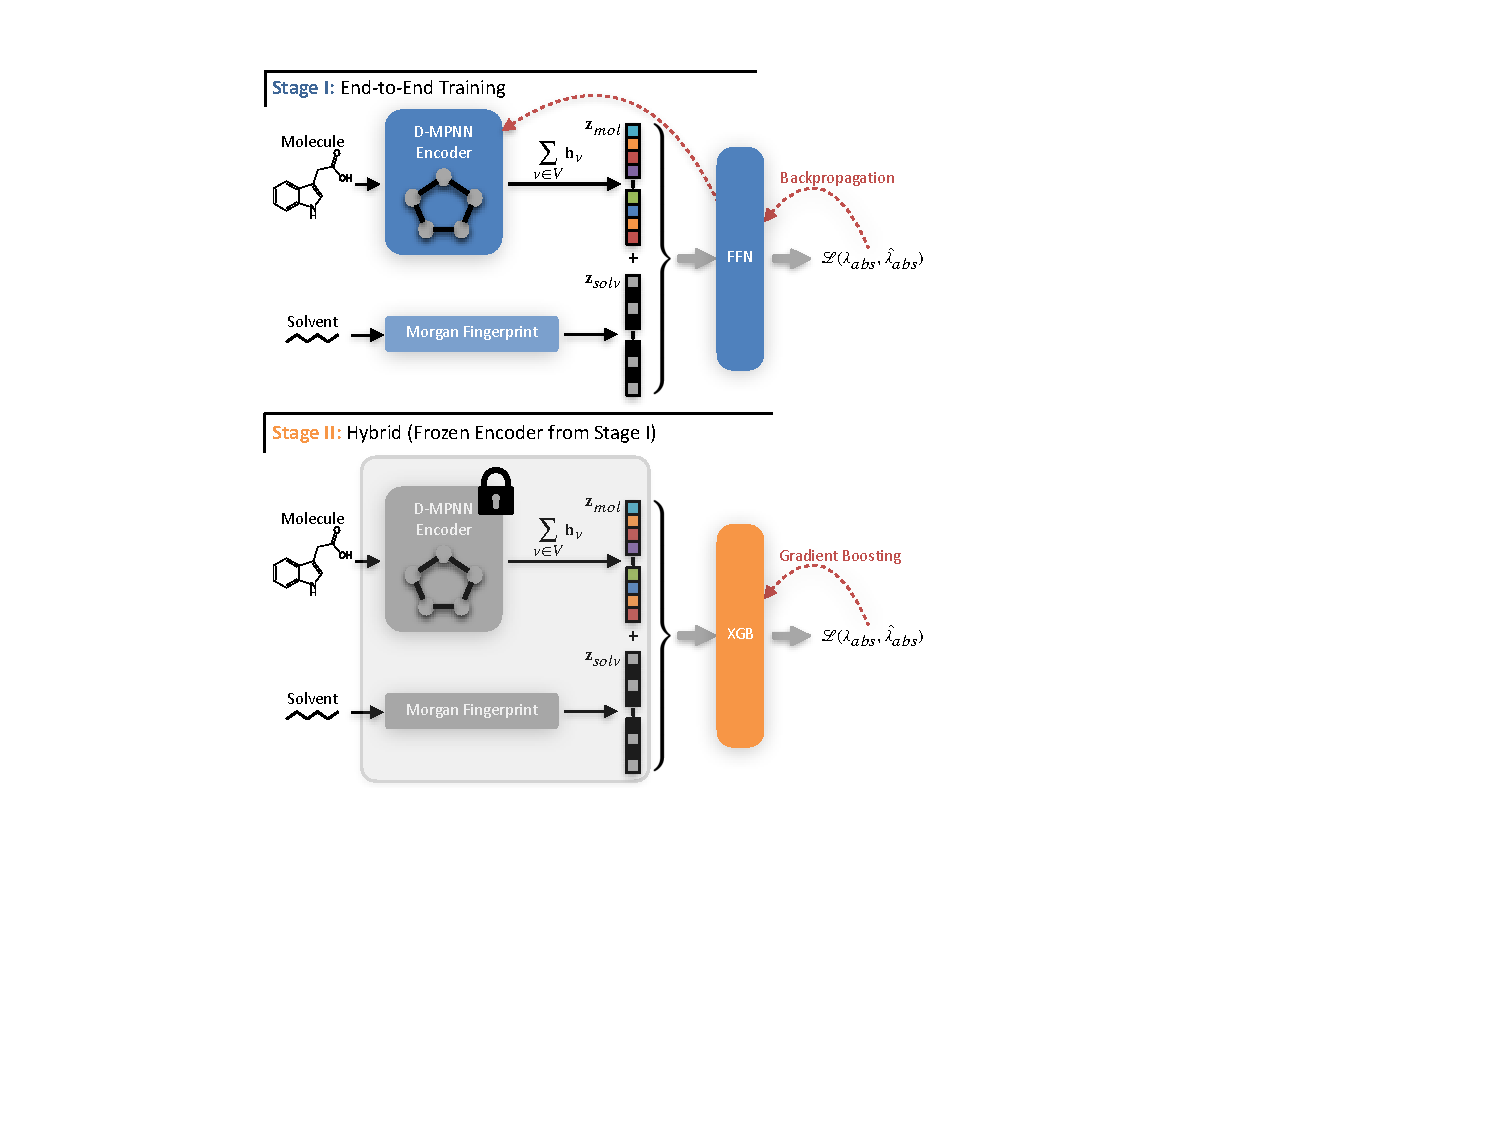
\includegraphics[width=0.8\linewidth]{figures/hybrid_end2end_architecture_schematic.pdf}
    \caption{\textbf{Two-stage hybrid modelling framework.} 
    \textbf{Stage I (Top):} A D-MPNN encoder maps the molecular graph to per-atom hidden states, which are aggregated via sum pooling to form a molecular representation ($\mathbf{z}_{\mathrm{mol}}$). This representation is concatenated with fixed solvent Morgan fingerprints ($\mathbf{z}_{\mathrm{sol}}$) and used to train a feedforward neural network (FFN) in an end-to-end manner, with gradients of the training loss propagated through both the FFN and encoder. 
    \textbf{Stage II (Bottom):} The pretrained D-MPNN encoder from Stage~I is frozen and reused to generate molecular representations ($\mathbf z_{\mathrm{mol}}$), which are again concatenated with solvent fingerprints ($\mathbf z_{\mathrm{sol}}$) and used as fixed features for an XGBoost head.}
    \label{fig:hybrid_schematic}
\end{figure}

We consider two modelling paradigms built upon the same D-MPNN encoder $\phi_{\theta}$ with parameters $\theta$, depicted in Figure~\ref{fig:hybrid_schematic}.

In the end-to-end paradigm, the molecular embedding $\mathbf z_{\mathrm{mol}} = \phi_\theta(G)
$ and solvent embedding $\mathbf z_{\mathrm{sol}}$ are concatenated and passed to a feedforward neural network (FFN) head $g_{\psi}(\cdot)$, and all parameters $\{\theta, \psi\}$ are optimized jointly:
\begin{equation}
\hat{y}_{\text{E2E}} = g_\psi(\mathbf z)
= g_{\psi}(\phi_{\theta}(G), \mathbf z_{\mathrm{sol}}).
\end{equation}

Given training data $\{(G_i,\mathbf z_{\mathrm{sol},i},y_i)\}_{i=1}^N$, parameters are learned by minimizing the empirical risk
\begin{equation}
\mathcal{L}(\theta,\psi)
=
\frac{1}{N} \sum_{i=1}^{N}
\ell\!\left(
y_i,
g_{\psi}(\phi_{\theta}(G_i), \mathbf z_{\mathrm{sol},i})
\right),
\end{equation}
where $\ell(\cdot,\cdot)$ denotes the task-specific loss function (mean squared error for regression in our experiments). Gradients of $\mathcal{L}$ are computed with respect to both encoder parameters $\theta$ and head parameters $\psi$.

This approach allows the learned representation to adapt directly to the prediction task but may introduce instability in low-data regimes due to the high-dimensional parameter space.

In the hybrid paradigm, we train the full encoder--head model, $g_{\psi}(\phi_{\theta}(G),\mathbf z_{\mathrm{sol}})$, end-to-end on the downstream task. After learning the parameters, we discard the FFN head $g_{\psi}(\cdot)$ and freeze the encoder $\phi_{\theta^*}(G)$, where $\theta^*$ indicates that the parameters are frozen. Predictions are then generated by a separate regression head $h_{\omega}$:
\begin{equation}
\hat{y}_{\text{hybrid}} = h_{\omega}(\phi_{\theta^*}(G),\mathbf z_{\mathrm{sol}}),
\end{equation}
where only the head parameters $\omega$ are optimized in the second-stage regression step. Decoupling representation learning from regression enables the use of models with different inductive biases, such as gradient-boosted trees, while ensuring that all comparisons are performed on the same frozen molecular embeddings augmented with identical solvent covariates.

\subsection{Downstream Regression via Gradient Boosting}
In our hybrid framework, we utilize XGBoost~\cite{chen2016xgboost} to serve as a regularized non-linear head for the frozen D-MPNN embeddings. Unlike the multi-layer perceptrons typically used in end-to-end GNNs, XGBoost constructs an additive ensemble of decision trees that incorporates explicit regularization on tree complexity (e.g., minimum split loss ($\gamma$) and leaf weights ($\lambda$)). This structural regularization is particularly advantageous in the data-limited regimes characteristic of experimental photophysics, where overparameterized neural heads are prone to overfitting.


\subsection{Baseline Models}

We evaluated several baseline approaches common to molecular property prediction. All baseline models were trained and evaluated using the same canonical data splits, fixed training subsamples, and evaluation protocols as the D-MPNN-based models.


\paragraph{Fingerprint-based baselines.}
As a classical cheminformatics baseline, molecules were represented using fixed-length Morgan fingerprints (radius 2, 2048 bits) computed with RDKit. Solvents were represented using separate Morgan fingerprints (radius 2, 1024 bits) which were concatenated with the molecular fingerprints. This concatenation strategy mirrors the solvent integration used in the D-MPNN and hybrid architectures, ensuring that all models have access to equivalent environmental context. To capture global physicochemical properties often missed by substructure fingerprints, we additionally explored augmenting these vectors with nine scalar descriptors: molecular weight (MolWt), octanol--water partition coefficient (MolLogP), topological polar surface area (TPSA), hydrogen bond acceptor and donor counts (HBA/HBD), aromatic and aliphatic ring counts, rotatable bond count, and the fraction of $sp^3$-hybridized carbon atoms ($f_{sp^3}$). These tabular representations were used to train a suite of regression models: ridge and polynomial regressions, Random Forests, and XGBoost models.

\paragraph{Physics-informed baselines.}
We evaluated the predictive utility of low-fidelity quantum-chemical (QC) descriptors derived from density functional theory calculations reported by Greenman \textit{et al.}~\cite{greenman2022multi}. In that work, molecular geometries were generated from SMILES strings and optimized using a multistage pipeline including semi-empirical tight-binding (GFN2-xTB), followed by DFT geometry optimization at the BP86-D3/def2-SVP level. TD-DFT calculations were then performed using the Tamm--Dancoff approximation at the $\omega$B97X-D3/def2-SVPD level of theory to estimate vertical excitation energies. For a subset of dye--solvent pairs, additional solvent-corrected TD-DFT calculations were carried out using the IEFPCM continuum solvation model. 

While these descriptors provide valuable physical signal, they require nontrivial QC calculations and are therefore substantially more expensive than purely data-driven representations. Accordingly, these baselines are included to contextualize the performance of learned representations relative to low-fidelity physics, rather than as a practical alternative in large-scale or low-latency settings.

Motivated by Tannir \textit{et al.}~\cite{tannir2024predicting}, we utilize the resulting HOMO--LUMO gap estimates as physics-informed descriptors. For molecules where this information was not available ($\leq 2\%$), we employ median imputation. These QC features were combined with fingerprint-based representations and used as inputs to the same downstream regression models, enabling direct comparison between learned representations, purely empirical features, and hybrid physics-informed baselines.

Finally, we evaluated a minimal parametric model motivated by Frontier Molecular Orbital (FMO) theory. Approximating the dominant optical transition energy by the energy gap between the highest occupied molecular orbital (HOMO) and the lowest unoccupied molecular orbital (LUMO), and invoking the Planck--Einstein relation ($E = hc/\lambda$), we fit an inverse-gap regression of the form:
\begin{equation}
\lambda_{\max} \approx \beta_0 + \beta_1 (\Delta \epsilon_{\text{H--L}})^{-1},
\end{equation}
to establish a predictive baseline rooted in first-principles physics. While this approximation neglects vibronic structure, excited-state relaxation, and explicit solvent reorganization, it provides a useful low-capacity benchmark against which more expressive learned representations can be evaluated.


For standard fingerprint- and descriptor-based baselines, we performed hyperparameter optimization using Optuna, utilizing the validation set for model selection. In contrast, the DFT-informed baselines were trained using default hyperparameters; consequently, we combined the training and validation sets for these models to maximize data utilization during fitting. Regardless of the training protocol, the test set was strictly reserved for final evaluation to ensure fair comparison across all architectures.

\subsection{Variance Decomposition Framework}
\label{subsec:var-decomp}

\begin{figure}[ht]
    \centering
    \begin{tikzpicture}[
    scale=0.7, transform shape,
    % Standardizes node styles
    encoder/.style={circle, draw=encodercolor, fill=encodercolor!10, thick, inner sep=2pt, minimum size=0.8cm},
    hpo/.style={rectangle, draw=hpocolor, fill=hpocolor!10, thick, rounded corners=2pt, inner sep=4pt},
    residual/.style={text=seedcolor, font=\small}, % Changed from \scriptsize\ttfamily
    % Tree geometry
    level 1/.style={sibling distance=2.4cm, level distance=1.2cm},
    level 2/.style={sibling distance=1.2cm, level distance=2.0cm},
    level 3/.style={sibling distance=0.7cm, level distance=1.4cm},
    edge from parent/.style={draw, -latex', gray!60, thick}
]

% Root node
\node[draw, rectangle, rounded corners=3pt, thick, inner sep=6pt, fill=gray!5] (root) {Training Data}
child {node[encoder] {$A_1$}
    % HPO Config 1 (j=1, i=1)
    child {node[hpo] {$B_{1(1)}$}
        child {node[residual] {$\varepsilon_{1(11)}$}} % Correct: k=1, j=1, i=1
        child {node[residual] {$\dots$}}
        child {node[residual] {$\varepsilon_{5(11)}$}} % Correct: k=5, j=1, i=1
    }
    child {node[gray!50, font=\Large] {$\dots$}}
    % HPO Config 5 (j=5, i=1)
    child {node[hpo] {$B_{5(1)}$}
        child {node[residual] {$\varepsilon_{1(51)}$}} % Correct: k=1, j=5, i=1
        child {node[residual] {$\dots$}}
        child {node[residual] {$\varepsilon_{5(51)}$}} % Correct: k=5, j=5, i=1
    }
}
    % Represent the gap to the 5th encoder
    child {node[gray!50, font=\Large, yshift=-0.5cm] {$\dots$} child[missing]}
% Encoder 5 branch (i=5)
child {node[encoder] {$A_5$}
    % HPO Config 1 (j=1, i=5)
    child {node[hpo] {$B_{1(5)}$}
        child {node[residual] {$\varepsilon_{1(15)}$}} % Correct: k=1, j=1, i=5
        child {node[residual] {$\dots$}}
        child {node[residual] {$\varepsilon_{5(15)}$}} % Correct: k=5, j=1, i=5
    }
    child {node[gray!50, font=\Large] {$\dots$}}
    % HPO Config 5 (j=5, i=5)
    child {node[hpo] {$B_{5(5)}$}
        child {node[residual] {$\varepsilon_{1(55)}$}} % Correct: k=1, j=5, i=5
        child {node[residual] {$\dots$}}
        child {node[residual] {$\varepsilon_{5(55)}$}} % Correct: k=5, j=5, i=5
    }
};

% Annotations for Levels (Vertical Labels on the Left)
\begin{scope}[xshift=-6.7cm, font=\small\bfseries\itshape, gray]
    % Added align=center to allow the \\ to work
    \node[align=center] at (0,-1.2) {D-MPNN Encoder \\ Representation};
    \node at (0,-3.2) {XGB HPO Config};
    \node at (0,-4.6) {Replicate Trainings};
\end{scope}

% % Legend Box - Placed Bottom Right
% \node[draw=gray!30, fill=white, rounded corners, thick, anchor=north west] at (4.5,0) {
%     \begin{tabular}{ll}
%         \textbf{Variance Source} & \textbf{Contribution} \\
%         \hline
%         \tikz\draw[encoder, minimum size=0.3cm] (0,0) circle (0.15); \ Encoder Seed ($A_i$) & \textbf{91.7\%} \\
%         \tikz\draw[hpo, minimum size=0.3cm] (0,0) rectangle (0.3,0.3); \ HPO Config ($B_{j(i)}$) & \textbf{2.9\%} \\
%         \textcolor{seedcolor}{$\bullet$} \ Residual Noise ($\varepsilon_{ijk}$) & \textbf{5.4\%} \\
%     \end{tabular}
% };

\end{tikzpicture}
    \caption{\textbf{Nested variance decomposition of predictive performance.}
    Schematic of the two-factor experimental design together with estimated variance components.}
    \label{fig:nested_anova_design}
\end{figure}
To quantify the sources of predictive variability in the hybrid encoder--head architecture, we adopt a two-factor nested random-effects variance decomposition. This framework partitions total performance variability into contributions arising from stochasticity in representation learning (encoder training), stochasticity in model selection at the head level (Bayesian hyperparameter optimization for XGBoost), and residual stochasticity associated with downstream regression given fixed hyperparameters.

We employ a balanced nested experimental design. Specifically, we train $I = 5$ independent D-MPNN encoders with different random initializations. For each frozen encoder, we perform $J = 5$ independent Bayesian hyperparameter optimizations for the XGBoost head, yielding distinct heads conditioned on that encoder. Finally, for each encoder--head pair, we train and evaluate the XGBoost model across $K = 5$ random seeds using the fixed hyperparameter set, capturing stochasticity arising from subsampling and tree construction. This design yields a total of $N = I \times J \times K = 125$ evaluations per dataset split.

Let $y_{ijk}$ denote the test-set RMSE obtained from the $i$-th encoder initialization ($i = 1, \dots, I$), the $j$-th regression head configuration nested within that encoder ($j = 1, \dots, J$), and the $k$-th replicate seed ($k = 1, \dots, K$). We model performance as
\begin{equation}
y_{ijk} = \mu + A_i + B_{j(i)} + \varepsilon_{ijk},
\end{equation}
where $A_i \sim \mathcal{N}(0, \sigma_A^2)$ captures encoder-level variability due to stochastic representation learning, $B_{j(i)} \sim \mathcal{N}(0, \sigma_{B|A}^2)$ captures variability induced by hyperparameter selection for the XGBoost head conditioned on a fixed encoder, and $\varepsilon_{ijk} \sim \mathcal{N}(0, \sigma_\varepsilon^2)$ represents residual variability associated with stochastic optimization and tree construction given fixed hyperparameters.

Variance components ($\sigma_A^2, \sigma_{B|A}^2, \sigma_\varepsilon^2$) were estimated using the ANOVA Method of Moments estimator for balanced designs (see Supporting Information for exact Expected Mean Squares formulas)~\cite{searle1992variance}. From these estimates, the proportion of variance attributable to the learned representation is computed as:
\begin{equation}
\eta_{encoder}^2 = \frac{\sigma_A^2}{\sigma_A^2 + \sigma_{B|A}^2 + \sigma_\varepsilon^2}.
\end{equation}


\subsection{Ensemble Modelling}

Following Greenman \textit{et al.}~\cite{greenman2022multi} we employ ensemble predictors to improve predictive stability and mitigate stochasticity arising from random initialization and training dynamics. Ensemble predictions are formed by averaging the outputs of $M$ independently trained models:
\begin{equation}
\hat{y}_{\text{ens}} = \frac{1}{M} \sum_{m=1}^{M} \hat{y}^{(m)},
\end{equation}
where each ensemble member $\hat{y}^{(m)}$ corresponds to a model trained with a distinct random seed.

In the hybrid paradigm, ensemble members correspond to independently trained encoder--head pipelines. In the end-to-end paradigm, ensemble members correspond to independently trained joint encoder--head models. Unless otherwise stated, ensemble predictions are used for all reported results.


\subsection{Transfer Learning and Fine-Tuning Protocols}

To evaluate the utility of learned representations in data-scarce regimes, we compare four distinct initialization and adaptation strategies. We report results for the following protocols:

\begin{enumerate} \item \textbf{Random Initialization (Baseline):} The D-MPNN encoder and prediction head are initialized randomly and trained end-to-end on the downstream dataset. \item \textbf{Zero-Shot Transfer:} The encoder and prediction head, pretrained on the largest dataset, are applied directly to the downstream dataset without any parameter updates. This serves as a reference for the off-the-shelf generalizability of the source model. \item \textbf{Two-Stage Fine-Tuning:} The encoder is initialized from weights pretrained on the source task and adapted to the target using a gradual unfreezing schedule. \item \textbf{Hybrid on Fine-Tuned Embeddings:} The D-MPNN is first fine-tuned via the two-stage protocol. The resulting adapted encoder is then frozen, and a gradient-boosted tree (XGBoost) head is trained on the extracted embeddings. \end{enumerate}

\paragraph{Two-Stage Fine-Tuning Schedule.}

For the fine-tuning strategies, immediate end-to-end optimization was found to cause training instability and catastrophic forgetting in ultra-low-data regimes ($N < 100$). To mitigate this, we employ a two-stage ``gradual unfreezing'' schedule.

Let $\theta$ denote encoder parameters and $\psi$ denote head parameters. 
Recall that $\mathcal{L}(\theta,\psi)$ denotes the empirical risk, which in this case can be written as
\[
\mathcal{L}(\theta,\psi)
=
\frac{1}{N} \sum_{i=1}^N 
\ell\!\left(
y_i,
g_{\psi}(\phi_{\theta}(G_i), \mathbf z_{\mathrm{sol},i})
\right).
\]

Starting from a pretrained checkpoint $(\theta_0,\psi_0)$, we first train only the head while the encoder remains frozen:
\begin{equation}
\textbf{Stage A (Warm-Up):}\quad 
\theta \leftarrow \theta_0, 
\qquad
\psi \leftarrow \arg\min_{\psi} \mathcal{L}(\theta_0,\psi),
\end{equation}
for $E_A$ epochs using a learning rate scaled by $\alpha_A$. This allows the head to align with the existing feature space before modifying the representation itself.


In the second stage, we unfreeze the encoder and fine-tune the full model end-to-end:
\begin{equation}
\begin{aligned}
\textbf{Stage B (End-to-End):}\quad
(\theta,\psi) &\leftarrow (\theta_A,\psi_A), \\
(\theta,\psi) &\leftarrow \arg\min_{\theta,\psi} \mathcal{L}(\theta,\psi),
\end{aligned}
\end{equation}
for $E_B$ additional epochs using a reduced learning rate scale $\alpha_B \ll \alpha_A$.
Unless otherwise noted, we use $E_A=30$ and $E_B=170$.


\subsection{Analysis of Learned Molecular Representations}

To analyze the structure of the learned molecular embeddings, we perform principal component analysis (PCA) on the frozen D-MPNN encoder outputs. PCA provides an orthogonal basis that captures dominant modes of variation in the learned embedding space while remaining invariant to rotations of the original coordinate system, which is essential given the non-identifiability of latent embedding axes across training runs.

All analyses are conducted on post hoc projections of the learned embeddings and do not influence model training. To account for stochastic variation across training seeds, PCA is performed independently for each encoder instance, followed by sign alignment of principal axes based on their correlation with an external physical reference quantity. This enables consistent aggregation and comparison of latent directions across seeds.

To probe chemical interpretability, aligned principal components are correlated with the independently computed physicochemical descriptors in Table~\ref{tab:chemical-descriptors} and target properties using Spearman rank correlation. These descriptors are not provided to the model during training and are used solely for interpretive analysis of the learned representation.

\begin{table}[ht]
\centering
\caption{Physicochemical descriptors computed via RDKit for latent space correlation analysis. These features were not used during model training but serve as independent probes for interpreting the learned representations.}
\label{tab:chemical-descriptors}
\begin{tabular}{ll}
\toprule
\textbf{Descriptor} & \textbf{Description} \\
\midrule
NumAromaticRings & Number of aromatic ring systems \\
FractionCSP3 & Fraction of \textit{sp}$^3$-hybridized carbon atoms \\
NumConjugatedBonds & Total number of conjugated bonds \\
LongestConjChain & Diameter (in bonds) of the conjugated-bond subgraph \\
TPSA & Topological polar surface area \\
NumHBA & Number of hydrogen bond acceptors \\
NumHBD & Number of hydrogen bond donors \\
ExactMolWt & Exact molecular weight \\
HeavyAtomCount & Number of non-hydrogen atoms \\
NumRotatableBonds & Number of rotatable single bonds \\
NumEtherO & Number of ether oxygen atoms \\
NumMethoxy & Number of methoxy substituents \\
NumMethylEster & Number of methyl ester groups \\
\bottomrule
\end{tabular}
\end{table}

